%% LyX 1.6.5 created this file.  For more info, see http://www.lyx.org/.
%% Do not edit unless you really know what you are doing.
\documentclass[10pt,twocolumn,english,times]{article}
\usepackage[T1]{fontenc}
\usepackage[latin9]{inputenc}
\pagestyle{empty}
\usepackage{graphicx}

\makeatletter
%%%%%%%%%%%%%%%%%%%%%%%%%%%%%% Textclass specific LaTeX commands.
\newenvironment{lyxcode}
{\par\begin{list}{}{
\setlength{\rightmargin}{\leftmargin}
\setlength{\listparindent}{0pt}% needed for AMS classes
\raggedright
\setlength{\itemsep}{0pt}
\setlength{\parsep}{0pt}
\normalfont\ttfamily}%
 \item[]}
{\end{list}}

%%%%%%%%%%%%%%%%%%%%%%%%%%%%%% User specified LaTeX commands.
%  $Description: Author guidelines and sample document in LaTeX 2.09$ 
%  $Author: ienne $
%  $Date: 1995/09/15 15:20:59 $
%  $Revision: 1.4 $
\usepackage{latex8}\usepackage{times}

%\documentstyle[times,art10,twocolumn,latex8]{article}
%------------------------------------------------------------------------- 
% take the % away on next line to produce the final camera-ready version 


%------------------------------------------------------------------------- 
\makeatother

\usepackage{babel}

\makeatother

\usepackage{babel}

\makeatother

\usepackage{babel}

\begin{document}

\title{RADICal: Really Awesome Distributed Internet Calendar (RADICAL)}

\maketitle
%\author{Lalith Suresh P.\\
%DEI\\
%Instituto Superior Tecnico\\
%Lisbon, Portugal\\
%suresh.lalith@gmail.com\\
%\and Marcus Ljungblad\\
%DEI\\
%Insituto Superior Tecnico\\
%Lisbon, Portugal\\
%marcus@ljungblad.nu\and Bruno Pereira\\
%DEI\\
%Insituto Superior Tecnico\\
%Lisbon, Portugal\\
%brunopereir4@gmail.com}


\thispagestyle{empty} 
\begin{abstract}
Shared calendar systems like Google Calendar are known to be an effective
way for people to schedule and coordinate events. In this project,
we design and implement RADICal, a peer-to-peer based distributed
calendar system. RADICal allows clients to make event reservations
amongst themselves in an almost decentralised manner with minimal
assistance from a central server. 
\end{abstract}

\section{Introduction}

The aim of this project is to design, implement and evaluate a shared
calendar system which has the following components: 
\begin{itemize}
\item Multiple clients, each with their own calendars, who may contact one
another to schedule events together. 
\item A centralised server which holds usernames and provides clients a
sequence number service. 
\end{itemize}
The rest of the paper is organised as follows: Section \ref{sec:systemarch}
describes the architecture of the different components of the system,
Section \ref{sec:Algorithms} explains the important algorithms that
underly RADICal, and Section \ref{sec:Conclusions} concludes the
paper.


\section{System Architecture\label{sec:systemarch}}

Since there is a Client and Server entity for this system, we describe
the architecture of each separetely. One of the main design goals
is to allow easy testability and debugging facilities within the system
in order to ease development. To a certain degree, we hope to achieve
this through classic 'printf' style debugging. Every class in PADICal
inherits from a class \texttt{PadiCalObject}, which has one virtual
method named \texttt{Debug()}. This method performs pretty printing
of internal state of an object, and follows the flow of logic through
the stack. All sub classes have to implement this method depending
on the kind of methods and state information they may hold. Additionally,
the NUnit framework is used during the development phase to ensure
methods do not misbehave when changes are introduced later. The \texttt{Debug()}
method of different objects comprising of a client or server can be
enabled via a configuration file or through some interfaces we can
provide to the UI of the client.

The client and the server follows a three-tier architectural decomposition.
From top to down, they are as follows: the interface layer, the services
layer, and the communications layer. In the sections below, we first
describe the client, the server, and the components of each of the
three layers that they comprise of.

In addition to the client and the server, a puppet master will be
introduced to facilitate testing. This component is not further discussed
in this paper.


\subsection{Client}

The client architecture is described in Figure. \ref{fig:clientarch}.
The working of the client has been decomposed into three layers, each
of which holds the appropriate working components. This is described
as follows:


\subsubsection{Interface Layer}

The client's interface layer comprises of the following: 
\begin{itemize}
\item \texttt{Client Interface}: The instantiation of this component handles
user inputs. The user can reserve events on the calendar, view the
calendar and connect/disconnect to the server. This interface is also
used by the puppet master to remotely control multiple clients. 
\end{itemize}

\subsubsection{Services Layer}
\begin{itemize}
\item \texttt{CalendarService}: This is the abstraction for the calendar
itself. The event reservation and commit protocols are implemented
within this component. 
\item \texttt{LookupService}: The Client performs lookups over the usernames
of other participants using this service. The (IP,Port) tuples returned
for each username are used to describe connections and remote object
invocations for every other component in the system. 
\item \texttt{ConnectionManager}: This component handles user login/sign-outs. 
\item \texttt{SequenceNumberService}: This service provides a unique sequence
number from the centralised servers. 
\end{itemize}

\subsubsection{Communications Layer}
\begin{itemize}
\item \texttt{SendReceiveMiddleLayer}: To abstract the underlying communication
process from the services, we use the \texttt{SendReceiveMiddleLayer}.
If there are multiple recipients to send a message to, this layer
uses the \texttt{GroupMulticast }abstraction, else, uses the \texttt{PointToPoint
}abstraction. It also acts as a demultiplexer (on the same lines as
Linux's {}``Layer 4/3 Demux\texttt{''}), to find the appropriate
service layer recipient for a particular message. 
\item \texttt{GroupMulticast}: This abstraction uses the \texttt{PointToPoint
}abstraction to deliver messages to a group of participants. 
\item \texttt{PointToPoint}: This abstraction uses a remote invocation to
send a message to a recipient. 
\end{itemize}
%
\begin{figure}[t]
\begin{lyxcode}
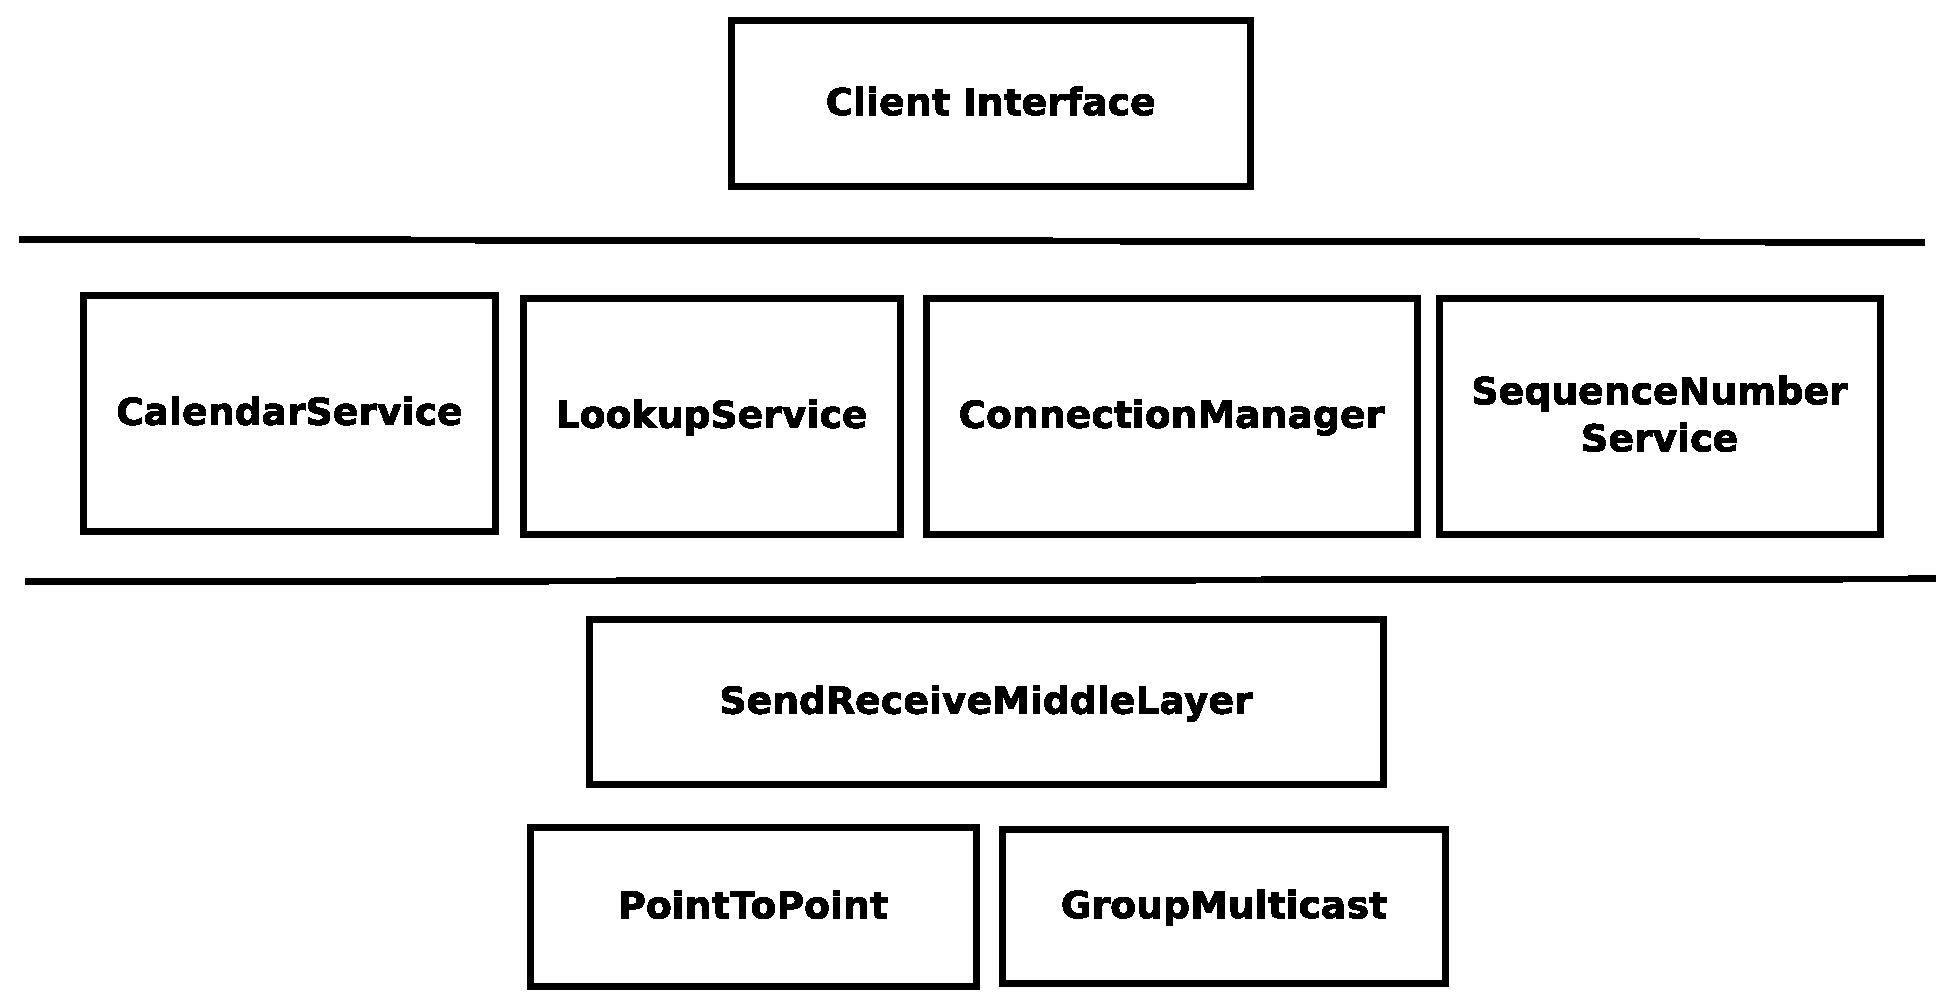
\includegraphics[scale=0.25]{client}~
\end{lyxcode}
\caption{Client Architecture. A three layer approach is used, with the following
stack: An interface layer (\texttt{Client Interface}), a service layer
(\texttt{CalendarService, LookupService, ConnectionManager, SequenceNumberService})
and a communication layer (\texttt{SendReceiveMiddleLayer, PointToPoint,
GroupMulticast}).\label{fig:clientarch}}

\end{figure}



\subsection{Server}

The Radical server consists of one master and three replicas. Each
replica is strongly consistent with the master and updated on each
write. In this section we describe the architecture of the servers,
including the replicas and its leader election process. The services
provided by the server are: a user to (IP, Port) lookup table and
sequence numbering. A server instance may be in one of two states:
master or replica. As a master, the instance is the primary and the
only node responsible for serving clients with data. We assume that
at most one instance may fail at any time during normal execution,
including the master. If the master instance becomes unavailable,
a new master is automatically elected among the three replicas. 
\begin{lyxcode}
%
\begin{figure}[t]
\begin{centering}
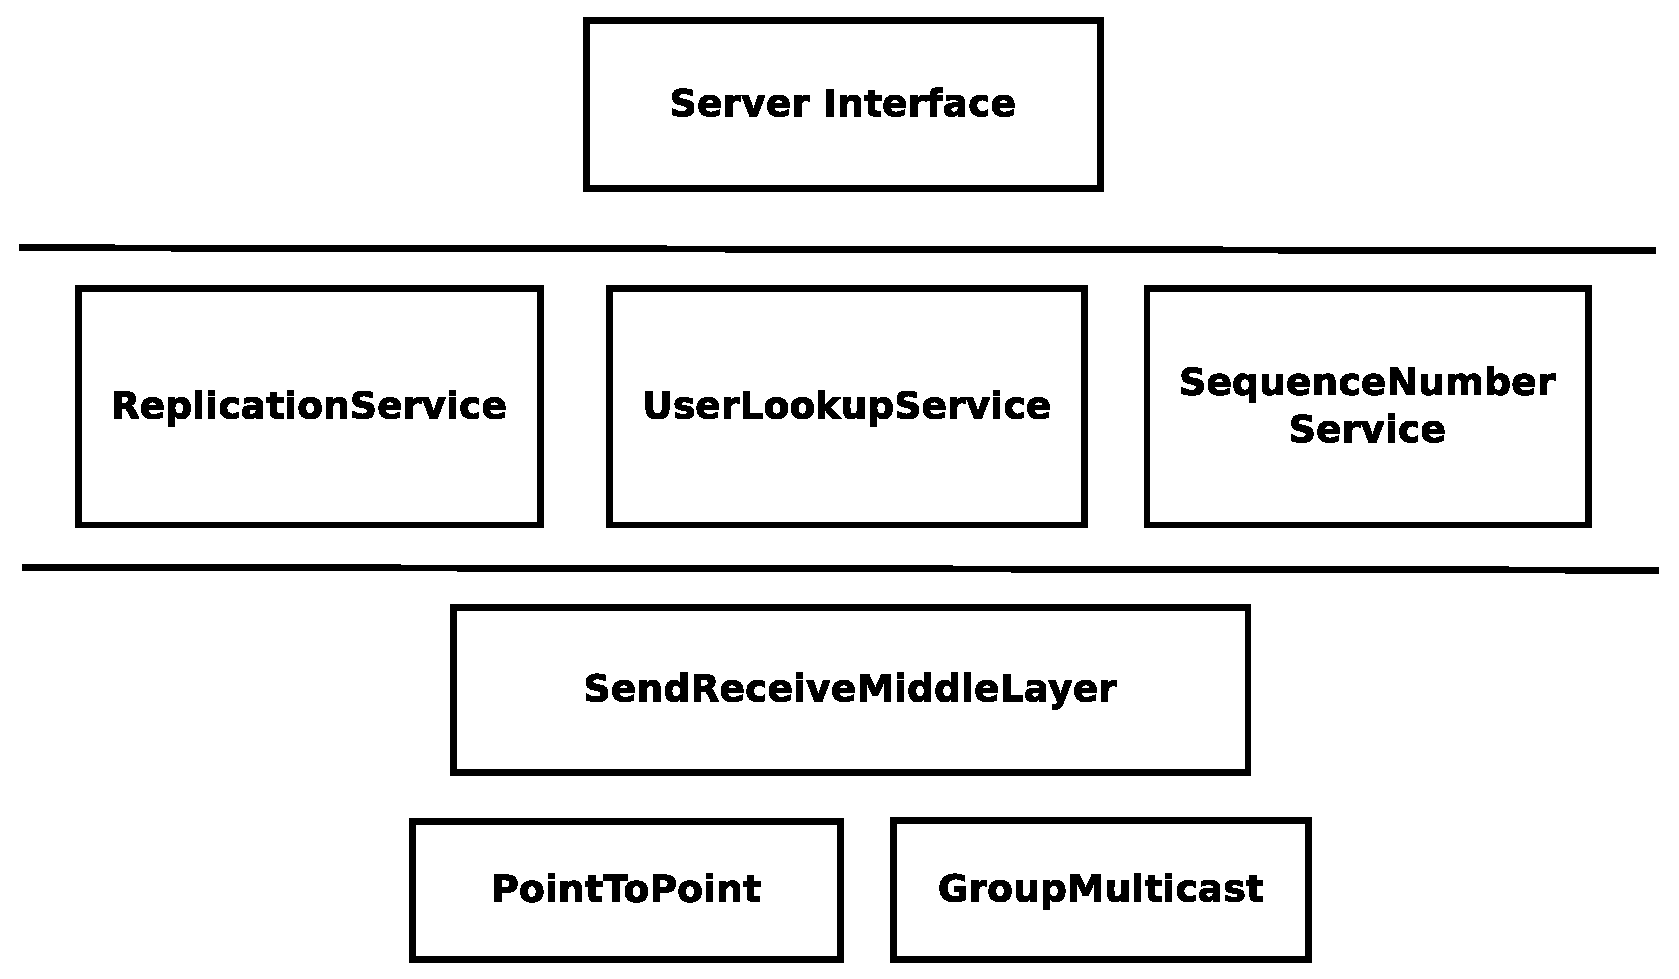
\includegraphics[scale=0.25]{server} 
\par\end{centering}

\caption{Server Architecture. A 3 layer approach is used, with the following
stack: An interface layer (\texttt{ServerInterface}), a service layer
(\texttt{ReplicationService, UserLookupService, SequenceNumberService})
and a communication layer (\texttt{SendReceiveMiddleLayer, PointToPoint,
GroupMulticast}).\label{fig:serverarch}}

\end{figure}

\end{lyxcode}

\subsubsection{Interface Layer}

The server's interface layer comprises of the following: 
\begin{itemize}
\item \texttt{Server Interface}: The instantiation of this class handles
user inputs. The user can view server state, the currently active
replica, and the currently logged on users. 
\end{itemize}

\subsubsection{Services Layer}
\begin{itemize}
\item \texttt{ReplicationService}: This is the abstraction for the strongly
consistent replication service. 
\item \texttt{UserLookupService}: This service handles both connect/disconnects
from the clients, and also provides the required username to (IP,
Port) lookup service for them. 
\item \texttt{SequenceNumberService}: This service provides a unique sequence
number to the clients. 
\end{itemize}

\subsubsection{Communications Layer}
\begin{itemize}
\item The components of the server communications layer remains the same
as that of the client. 
\end{itemize}

\section{Algorithms\label{sec:Algorithms}}


\subsection{Client Side: Reservation/Commit Protocol}

The reservation protocol follows the steps as outlined in the project
description. Once a client is in the tentatively booked state for
a particular event slot, it executes the commit protocol.

We have opted to use a 3-phase commit algorithm \cite{Skeen:1983:FMC:1313337.1313750}
with slight modifications to account for the specifics of the scenario
being tackled (orderly leaves by nodes for instance). It works as
follows: 

%
\begin{figure}
\begin{lyxcode}
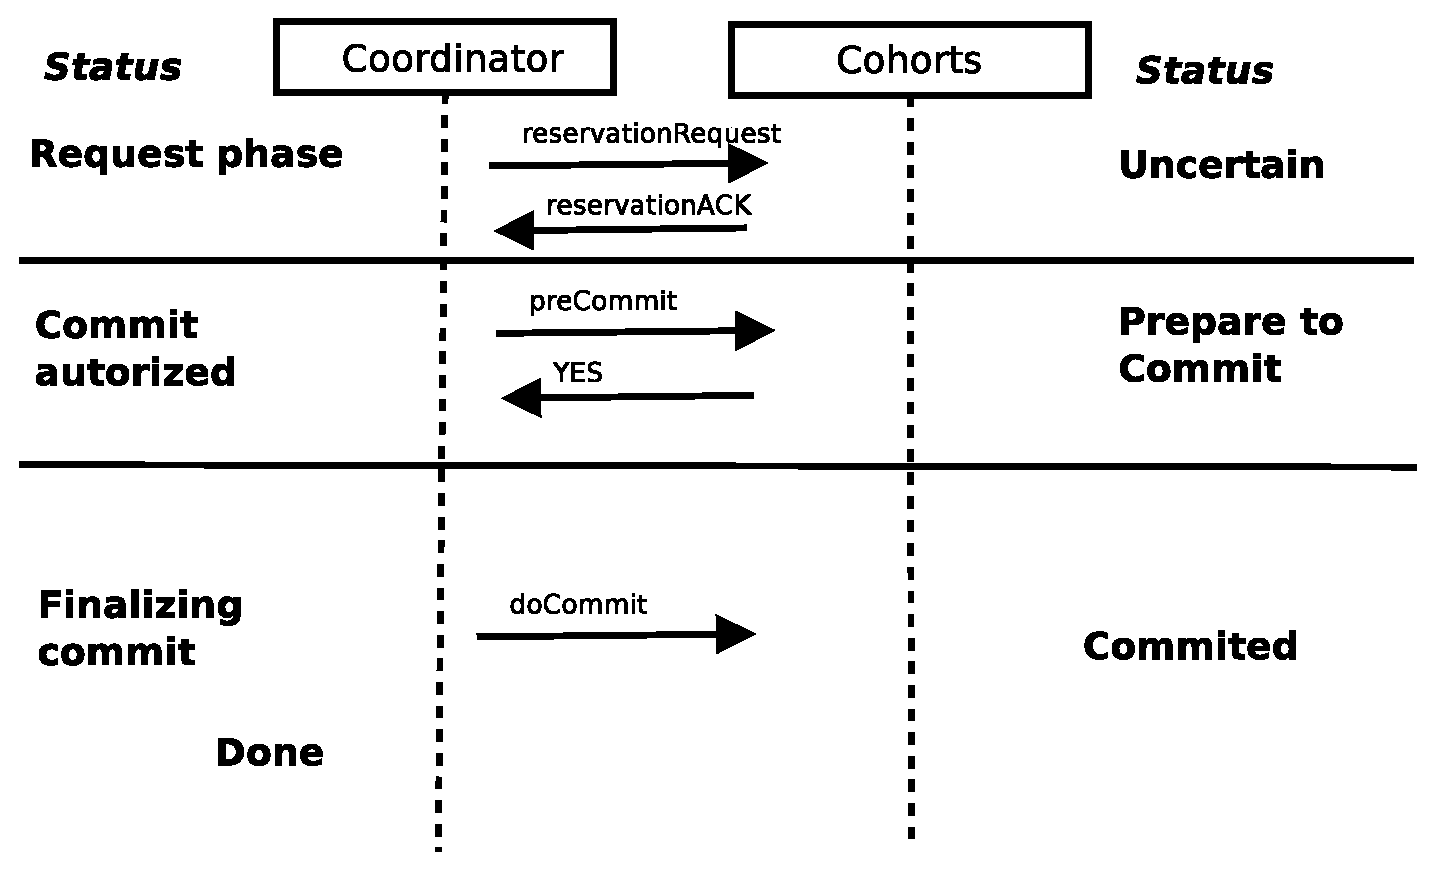
\includegraphics[scale=0.25]{3pcommit}
\end{lyxcode}
\caption{Client side 3 phase commit with modification for partition tolerance.}



\end{figure}

\begin{itemize}
\item Coordinator side (initiator of the event reservation):

\begin{enumerate}
\item The coordinator sends out reservation requests to all nodes. Nodes
then send their preferred list of slots (if any) to the coordinator
with RESERVATION-ACK messages, or decline the reservation request
with a RESERVATION-NACK message. If all nodes send RESERVATION-ACK
messages, the coordinator picks the first common slot agreed to by
the cohorts according to its preference and sends out a PRECOMMIT
message to all cohorts.
\item The coordinator then collects YES or ABORT messages from all the cohorts
depending on whether or not they agree to proceed further in the reservation.
\item If all nodes agree with a YES message, then the coordinator sends
all the cohorts a DOCOMMIT message, and it updates the reservation
status to COMMITTED, and the particular calendar slot to ASSIGNED.
This completes the reservation.
\item If at least one node sends an ABORT message, the coordinator aborts
the reservation, and sends out ABORT messages to all the cohorts,
causing them to abort as well.
\end{enumerate}
\item Cohort side (other participants in reservation):

\begin{enumerate}
\item The cohort receives a reservation request for a list of slots. If
it has at least one free slot from the list, then it responds with
those free slots in the form of a RESERVATION-ACK message. If none
of the requested slots are free, then the cohort responds with a RESERVATION-NACK.
\item If the cohort gets a PRECOMMIT message from a coordinator, then it
implies that all cohorts have responded for the reservation request
positively. The cohort then makes the following check:

\begin{enumerate}
\item If pre-commit-queue is empty, and there is no reservation under lock,
then lock this reservation and respond with a YES message.
\item If there is a reservation under lock, then add to the pre-commit-queue
if the reservation ID is newer than that under the lock. Do not respond
with any message at this point.
\item Attempt to abort newer reservation in favour of older one. This is
done by sending an ABORT message to the coordinator, and then waiting
for a response from the coordinator before performing the ABORT itself.
If the cohort receives a DOCOMMIT message after sending an ABORT,
it commits the currently locked reservation and aborts all reservations
in the queue.
\end{enumerate}
\item If the cohort receives a DOCOMMIT message, then commit the reservation
and change the respective slot's status to ASSIGNED.
\end{enumerate}
\end{itemize}
Step 2.c protects against a potential deadlock situation which can
arise as follows:
\begin{enumerate}
\item Let there be a reservation R1 coordinated by node A, involving nodes
B and C. Let there also be a reservation R2, coordinated by D, which
has occured later than R1, involving nodes B and C as well.
\item One possible scenario that can arise is as follows: B has a lock on
reservation R1, and has R2 in its pre-commit queue. C has a lock on
reservation R2 and now receives the pre-commit message for R1. At
this point, note that reservation R2 cannot proceed since node B never
sent a YES message for R2, even though node C already has. But in
this event, node C sends out an ABORT message to its coordinator D,
causing it to abort reservation R2. Node C then promotes reservation
R1 from its pre-commit queue to its lock position, and responds with
a YES message to node A for reservation R1.
\item The older reservation R1 thus advances.
\end{enumerate}

\subsection{Server Side: Leader Election and Replication}


\subsubsection{Leader Election}

All instances of a server knows about all other server instances.
Each instance has a unique id. Since the number of servers never exceeds
four, each server regularly emits a heartbeat to let the other servers
know it is alive. It is assumed that at most one server may fail at
any time. During the bootstrap of a server, each instance will select
the server with the highest ID (IP-Port combination) to be the leader.
Our leader election process is based on the Bully algorithm proposed
by \cite{GarciaMolina}. In case of a server failure, when any other
instance suspects that a server is unavailable, it will send a proposal
to all other servers that X is unavailable. If all others agree, the
server with the next highest ID is elected the new leader. The leader
is selected in a round-robin fashion.

To handle network partitions, a server may only become a leader if
it is part of the cluster with a majority of the servers. In case
each cluster is of equal size, the cluster with the current leader
will remain/elect the leader. This assumes that the leader's failure
and the 2-2 partition does not happen simultaneously. Clients trying
to contact the minority cluster will not get any replies, and according
to the round-robin selection scheme, will eventually pick a server
from the majority cluster.


\subsubsection{Replication}

In the interface above, three of the interfaces are considered writes.
Since we want to maintain a strong consistency among the replicas,
the master instance will propagate a write to all replicas before
replying to the client. The propagation is assumed to be synchronous
and utilises the broadcast component of the communication layer described
earlier. Thus, a server which receives a request will block until
it receives an acknowledgement from all correct replicas. The hit
this takes on performance can be justified by the fact that a replicated
set of servers which are highly available would most likely be on
a rack with a high bandwidth inter-connect. A replica is considered
alive as long as a heartbeat has been received within the given timeframe.

In case a replica, i.e an instance which is not the leader, gets an
unexpected request from a client it will query the leader for the
data, and retransmit the response to the client. Before propagating
write requests to replicas, the leader maintains a log of all write
records. When a server fails, and after a new leader is elected, the
server instances will synchronize to ensure that the user lookup table
and sequence number is aligned. Each write to the user lookup table
updates a logical timestamp, such that ordering can be guaranteed.


\subsection{Possible Optimisations}
\begin{itemize}
\item Minimising username lookups from the client side by using a cache
(on the same lines as a DNS cache). 
\item In the scheme for committing a reservation, it is possible that two
clients can be part of two reservation sequences, and each of them
can abort each other's sequences. This is a safety measure, but it
is possible to use a tie-breaking system at the tentatively booked
phase. 
\item It is possible to only consider a subset of acknowledgements when
propagating writes in the server cluster, thus improving performance. 
\end{itemize}

\section{Evaluation}
Results
- quantitative
  run all traces: number of msgs, avg size of msgs (max deviation?), commit ratio

- qualitative
software architecture obeyed 
limitations of commit protocol

Analysis
- performance
- what went well... maybe unnecessary
- what could be improved: 
  pass coordinator function to another node to make case 8 work (with forwarding) 
  


\section{Conclusions\label{sec:Conclusions}}

In this paper, we have presented the design and architecture for RADICal,
a peer-2-peer distributed internet calendar service. The design is
made with testability in mind. The algorithms have been designed for
handling partition tolerance on the client side, and strong consistency
with availability on the server side.

\bibliographystyle{latex8}
\bibliography{latex8}

\end{document}
